%% The following is a directive for TeXShop to indicate the main file
%%!TEX root = diss.tex

\chapter{Background}
\label{ch:background}

\section{IoT Architecture}
Figure \autoref{fig:arch} shows a typical architecture of an IoT system which is based on the architectures defined in previous studies~\citep{towardsIoTDefinition,stojkoska2017review,vcolakovic2018IoT,eclipse2016three}. 

\subsection{Device Layer}
The device layer at the bottom, which is the closest component to the physical world, includes smart programmable things interacting with the environment through their embedded sensors and actuators. Some IoT devices employ light embedded operating systems (e.g. contiki, RIOT, TinyOS) that have support for various programming languages allowing developers to write embedded code, such as application-specific logics for IoT devices, on top of the device OS~\cite{javed2018OS}. IoT operating systems aim to hide the minor details of the device hardware and provide basic OS tasks, like memory management and real-time scheduling, efficiently\cite{javed2018OS}. On the other side of spectrum, bare metal IoT devices run the embedded code directly on their hardware processor. Underlying details of the device hardware is usually abstracted by hardware abstraction layer (HAL) to enable access for the operating system to various hardware components like GPIO, and serial interfaces\cite{eclipse2016three}. In addition, IoT devices should have a connectivity capability which includes drivers, external libraries, and communication protocols to allow them communicate over a local wired or wireless communication, which allows devices to be remotely controlled by external entities.


 \begin{figure}[t]
  \centering 
   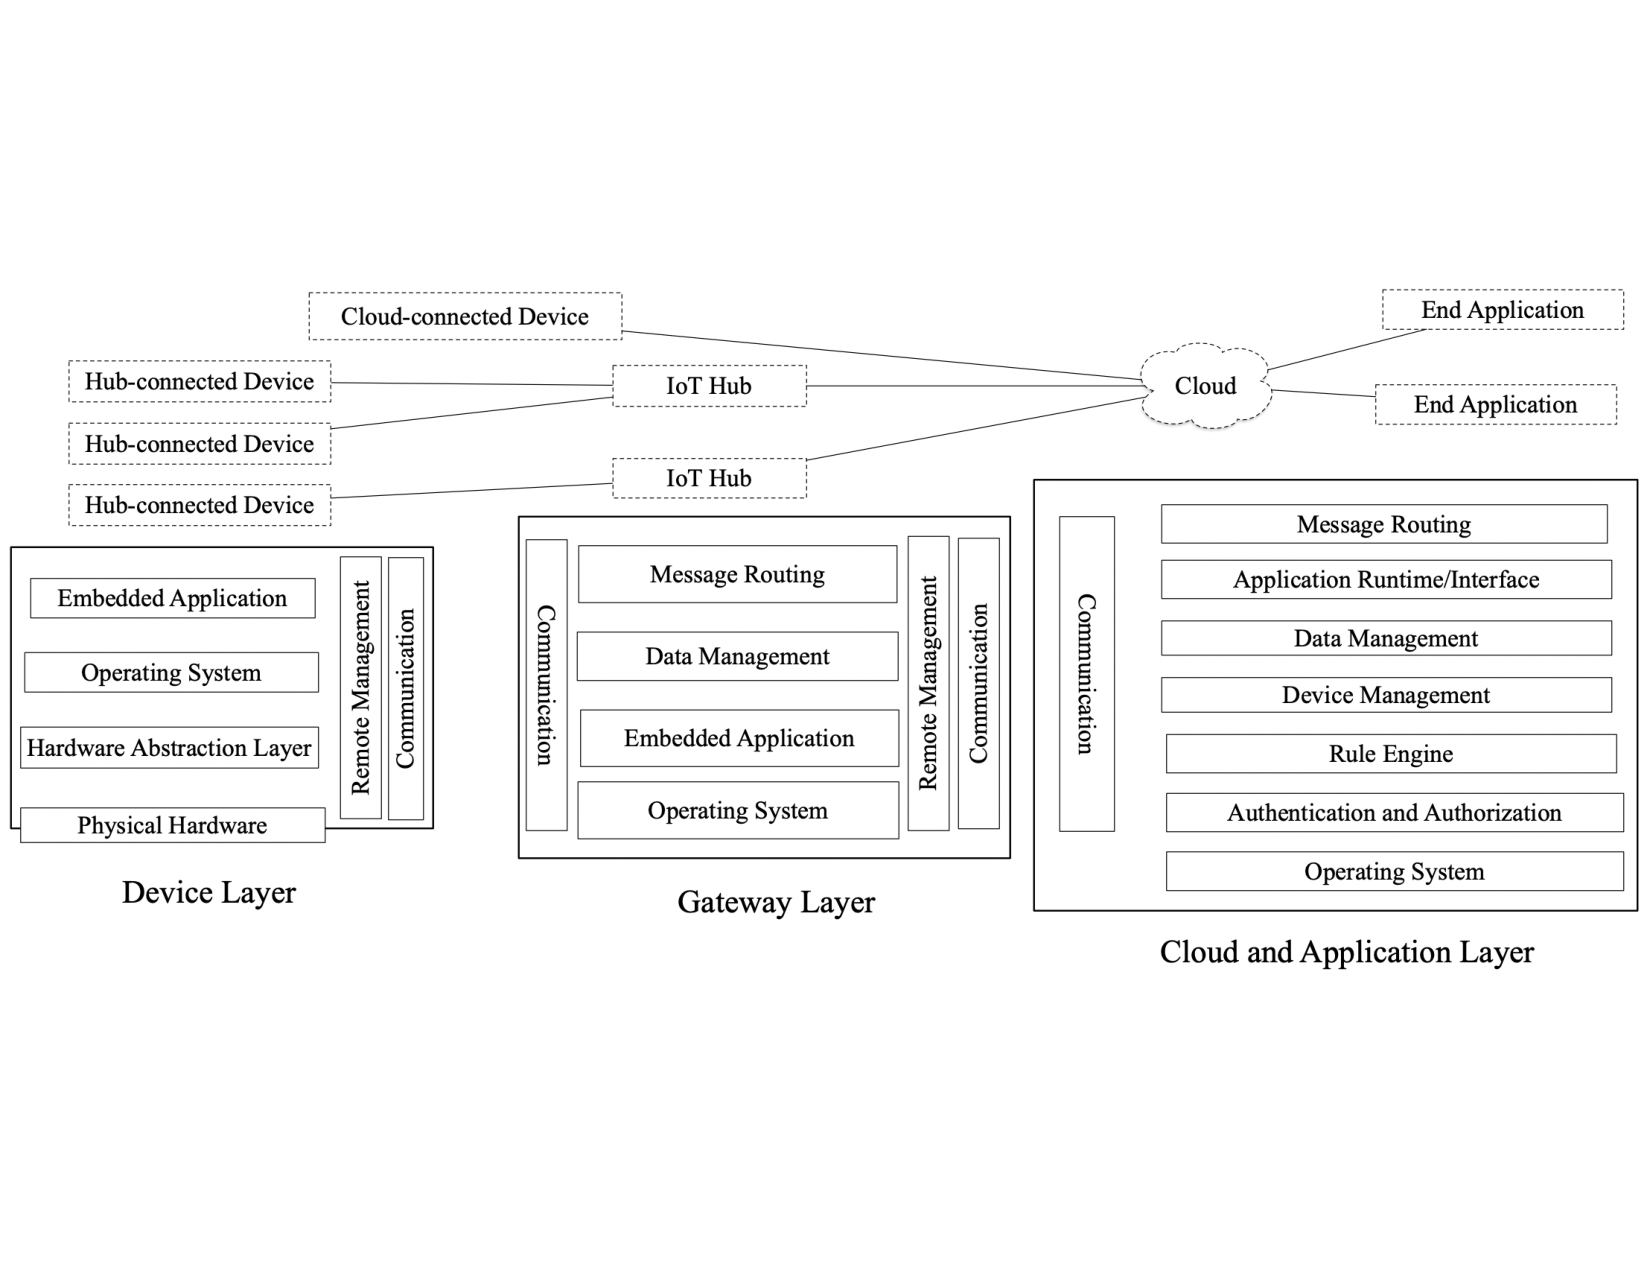
\includegraphics[width=\linewidth]{./imgs/arch1.pdf}
  \caption{A typical layered architecture of IoT systems and software stack for each layer}
  \label{fig:arch}
\end{figure}


\subsection{Gateway Layer}
This layer contains gateway devices with fewer resource constraints with the ability to handle telemetry data collection, processing, and routing locally on the edge. Gateway devices can handle the device-device and device-cloud interoperability by interpreting diverse communication protocols such as MQTT, CoAP, and HTTP~\cite{tschofenig2014architectural}. 

The IoT gateway devices have less resource constraint and the ability to handle telemetry data collection, processing, and routing locally on the edge. These devices can offer secure communication with remote systems since they can employ full-stack communication protocols and security mechanisms\cite{bormann2014terminology}.

There are different types of IoT devices based on their processing, power, and storage capabilities~\cite{bormann2014terminology} which affects the way they communicate with the cloud systems over the internet. Gateway-connected devices, as the name suggested in~\cite{securityUsenix2019}, are designed to do a limited functionality due to their constrained resources, thus, they rely on gateway devices for specific application purposes, data management, or secure communication with remote cloud systems~\cite{bormann2014terminology}. On the other hand, cloud-connected devices have the ability to talk directly to the cloud by employing protocols designed specifically for constrained devices like Constrained Application Protocol (CoAP). They should have enough resources to do basic data pre-processing and to apply security mechanisms by themselves without the help of a gateway device~\cite{stojkoska2017review,securityUsenix2019}. Gateway devices can handle the device-device and device-cloud interoperability by interpreting diverse communication protocols of both sides\cite{vcolakovic2018IoT}. Both types of IoT devices allow higher level components to control, monitor, and upgrade them remotely~\cite{eclipse2016three}.

\subsection{Cloud and Application Layer}
Remote IoT cloud servers accumulate and process all telemetry data, and communicate with a large number of heterogeneous gateway or cloud-connected devices to control and monitor them remotely. IoT cloud servers rule engine lets users write automation logic between IoT devices to define interoperability behaviours of the IoT system~\cite{securityUsenix2019}. 

End users and end applications can monitor the telemetry data and device status, and send commands to IoT devices to control and configure them remotely from the cloud. Usually, external end users and end applications should be authenticated and authorized in the cloud to be able to use these services. Some IoT cloud providers offer an interface for third-party applications, and allow users to run custom code in the application runtime environment on top of the cloud services\cite{vcolakovic2018IoT} and also allow them to have direct access to the analytical data via various visualizations and customized dashboards.


\section{Motivation}
\afterpage{%
 \begin{figure}[t]
  \centering 
   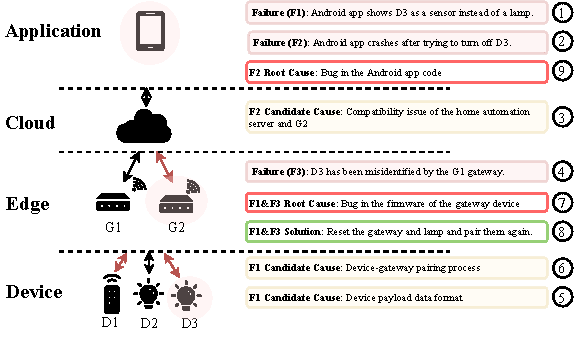
\includegraphics[width=\linewidth]{./imgs/motiv.pdf}
  \caption{The steps IoT developers have went through to find the root cause of a real IoT bug occurred in~\cite{iotbug:290}.}
  \label{fig:arch}
\end{figure}
\clearpage
}

Dealing with bugs and their causes in IoT systems is not a trivial task for developers. Below, we will do an in-depth investigation of a real bug report in an IoT system as an example of how dealing with bugs can be time-consuming for IoT developers. In addition to discussing the bug, we also showcase some challenges IoT developers have went through while debugging. 

Figure \ref{fig:arch} shows (on the right side) the steps that IoT developers have taken to find the root cause of the bug report PYTRADFRI/135~\cite{iotbug:290}. This bug occurred in a smart home environment where different devices should be connected to a home automation server with the help of a gateway device.


Based on developers' discussions, the first manifestation of this bug happens at the application layer. A light bulb device (D3) is mistakenly recognized as a sensor device (F\textsubscript{1}) as the user adds it, and also the Android app crashes (F\textsubscript{2}) once it tries to turn the light bulb off (step 1 and 2). Initially, the developers suspected the root cause of the bug to be the incompatibility of a gateway library with the home automation server (step 3).


However, further investigation of the failure in the edge layer (step 4), revealed that the gateway misidentifies D3 as a remote controller (F\textsubscript{3}). Since the gateway in this system relies mainly on a specific format of response data from devices to identify their types properly, potential inconsistencies of the payload data from the subject device were also investigated (step 5). In addition, developers should consider the device type, model, manufacturer, and the firmware version to detect possible breaking changes in the device firmware by the device manufacturer. 

But, further investigation eliminated the possibility of the device payload data as the root cause as some users reported that the same setting has not caused any issue for them. As the next step developers tried pairing in different circumstances (step 6), since the device battery and distance to the gateway could affect the pairing process. After none of the candidate causes showed as the potential reason for the bug, the root cause was identified as an external bug in the firmware of the G2 gateway device (step 7) and resetting both the device and the gateway and pairing them again solved the issue (step 8). But surprisingly F\textsubscript{2} continued to exist. After monitoring the data that the app receives via Wireshark, the root cause of F\textsubscript{2} was identified as a fault in the Android app code (step 9).

This example shows how one bug in the firmware of the gateway device, can make a lamp in the device layer useless, and cause observable failures in edge and application layers. Distribution of IoT failures and their candidate causes in different layers of IoT required a wide range of development skills from developers, as we could see that developers have to both investigate low-level firmware code and debug high-level application code to find the root cause of a single bug. Also dealing with behaviours of diverse devices such as comparing their payload, and depending on naive debugging practices such as monitoring network traffic, make it extremely hard for developers to deal with IoT bugs. Another challenging factor that we observed in this case study, is the interference of physical factors like the battery and the distance of the IoT devices from the gateway devices, which makes the debugging process rather time-consuming and complex.

Despite these compelling challenges, previous studies~\cite{hnat2011hitchhiker,corno2019challenges,stojkoska2017review,chen2017application,IoTOSBugs} do not take into consideration real-world experiences of IoT developers. In this paper, we aim to provide a systematic and generalized understanding of bugs and challenges in IoT by mainly considering IoT developers' experiences.

\endinput

